\section{Simulationen zur Steuerung von Flugobjekten}
\subsection{Flugdynamiken}
Die Simulation des Quadrokopters stellt eine Simulation eines Flugkörpers mit drei Rotations- und drei Translationsbewegungen und demnach insgesamt sechs verschiedenen Freiheitsgraden dar. \footcite[Vgl.][S. 2]{Koch}
Ein Quadrokopter ist dabei ein fester Körper mit vier befestigten Rotoren welche sich ausschließlich in eine Richtung drehen und positiven Schub in die Z-Achse des Körpers ausüben können. \footcite[Vgl.][S. 3]{Molchanov}
Die vier Rotoren werden als + oder X Konfiguration entweder direkt in Richtung der X- und Y-Achse (+), oder um 45° gedreht (X) an der Drohne befestigt. \footcite[prenote][S. 2]{Koch}
Jede Bewegung der sechs verschiedenen Arten wird durch die unterschiedliche Steuerung, der im Fall des Quadrokopters, vier Rotoren getätigt.
Eine unterschiedliche Ansteuerung der Rotoren und den demnach verschieden starken Auftrieben resultiert in den drei Rotationsbewegungen Rollen, Nicken und Gieren. \footcite[Vgl.][S. 2]{Koch}
\begin{figure}[htb]
    \centering
    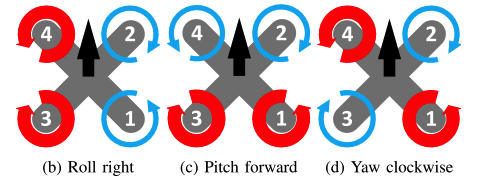
\includegraphics[height=3cm]{lib/graphics/Drone axis.png}
    \caption[Rotationsbewegungen eines Quadrokopters]{Rotationsbewegungen eines Quadrokopters\footnotemark}
    \label{abb:drone axis}
\end{figure}
\footnotetext{Enthalten in: \cite[][S. 2]{Koch}}

Rollen wird wie aus Abbildung drei hervorgeht durch unterschiedlichen Auftrieb der zwei linken oder rechten Rotatoren, das Nicken durch Unterschiede der vorderen und hinteren Rotatoren hervorgerufen.
Das Gieren bzw. die Rotation um die Z-achse wird durch die stärkere Rotation der sich im Uhrzeiger drehenden oder der sich gegen den Uhrzeiger drehenden Rotoren bewerkstelligt. 